% Chapter Template

\chapter{Experimental Results} % Main chapter title

\label{Chapter6} % Change X to a consecutive number; for referencing this chapter elsewhere, use \ref{ChapterX}

\lhead{Chapter 6. \emph{Experimental Results}} % Change X to a consecutive number; this is for the header on each page - perhaps a shortened title

\section{Introduction}
    We consider our target platform to be a single compute node comprising an NVIDIA GTX-970 GPU card and a Quadcore Intel i5-4690K CPU which was also used for our motivational example. We perform our experiments using DAGs pertaining to the Transformer Neural Network \cite{DBLP:journals/corr/VaswaniSPUJGKP17} which is a popular inference pipeline employed in Natural Language Processing (NLP) tasks. The primary objective of the transformer is to produce context aware embeddings for each word of a sentence to be used in downstream NLP tasks such as Named Entity Recognition and Neural Machine Translation. A diagrammatic representation of a general transformer architecture is depicted in Fig. \ref{fig:transformer}. In the following section, we give a detailed description of the Transformer architecture
\section{The Transformer}
	\par A transformer is based on the standard encoder-decoder architecture used in sequential learning tasks. The input to the transformer is a sentence matrix $X = [w_{1}^\intercal,w_{2}^\intercal,w_{3}^\intercal....w_{n}^\intercal]$ where $w_i \in \mathbb{R}^d$ represents an embedding vector for each word in the sentence. The matrix $X$ undergoes transformations through each layer in the encoder and decoder before yielding the target vector $Y$. The operations in each of the layers are similar in nature and thus for the purpose of our experiments, we focus on the computation involved in one such layer. 
	\par The transformer uses an attention mechanism and scores each word in the sentence. The scores represent the importance of any word in the sentence relative to other words. This is achieved by a series of matrix transformations through a mechanism called multi-headed attention.  A transformer head $h$ represents a series of linear algebra operations operating on the sentence matrix $X$ for generating a contextual embedding matrix $Z_h$ comprising contextual embedding vectors for each of the $n$ words in the sentence. Each layer in the transformer comprises multiple attention heads that operate in parallel. 
	\par Each head $h$ is characterized by four parameter weight matrices $W_h^Q,W_h^K, W_h^V $and $W_h$. 
	The computation involved in each head $h$ is represented by the DAG on the right hand side of Fig. \ref{fig:transformer}. This was the same DAG used in the motivational example in Chapter \ref{Chapter2}. It can be observed that the sentence vector $X$ typically undergoes 3 parallel GEMM transformations with the weight matrices $W_h^Q,W_h^K, W_h^V $ to generate Query $Q$, Key $K$ and Value $V$ matrices respectively. The contextual embedding matrix $C = [h_{1}^\intercal,h_{2}^\intercal,h_{3}^\intercal....h_{n}^\intercal]$ is produced as follows.
	$$C = softmax(Q \times K^\intercal) \times V$$ 
	Finally, the output $Z_h$ is obtained by the GEMM operation $CW_h$. The outputs of each of these heads are concatenated to produce the final contextual embeddings for the sentence. The output of each layer is passed as input to the following layer similar to any neural network based inference pipeline.
	
	\par In the recent past, Transformer \cite{DBLP:journals/corr/VaswaniSPUJGKP17} neural networks have proven to yield signficantly better results than the state of the art Recurrent Neural Network (RNNs) architectures such as LSTMs \cite{hochreiter1997long}, where given a sentence $ S = \{w_1,w_2,w_3....,w_n\} $, and $\forall i \in [1,n]$  \cite{NIPS2013_5021} \cite{Pennington14glove:global} of the sentence, the RNNS produced  context aware embeddings $h_i$ in a recursive manner as follows.
	$$
	h_i = f(h_{i-1},w_i;\theta)
	$$
	$$
	h_1 = \vec{0}
	$$
	The recursive formulation of $f$ enforces that $h_{i}$ can only be computed once the set of embeddings $\{h_0,h_1,....h_{i-1}\}$ have been computed. In contrast, transformer architectures offer ample scope for parallelization.
	A single transformer layer typically comprises, 8 or 16 heads and thus a maximum of $16*3=48$ matrix computations can execute in parallel given the hardware resources. For our experiments, we design a single layer of the transformer network using the specification file format offered by {\em PySchedCL}. As component kernels, we use kernels that are readily available from the Polybench \cite{polybench}, NVIDIA OpenCL \cite{nvidia} benchmark suites. 
	\begin{figure}[ht]
		\centering
		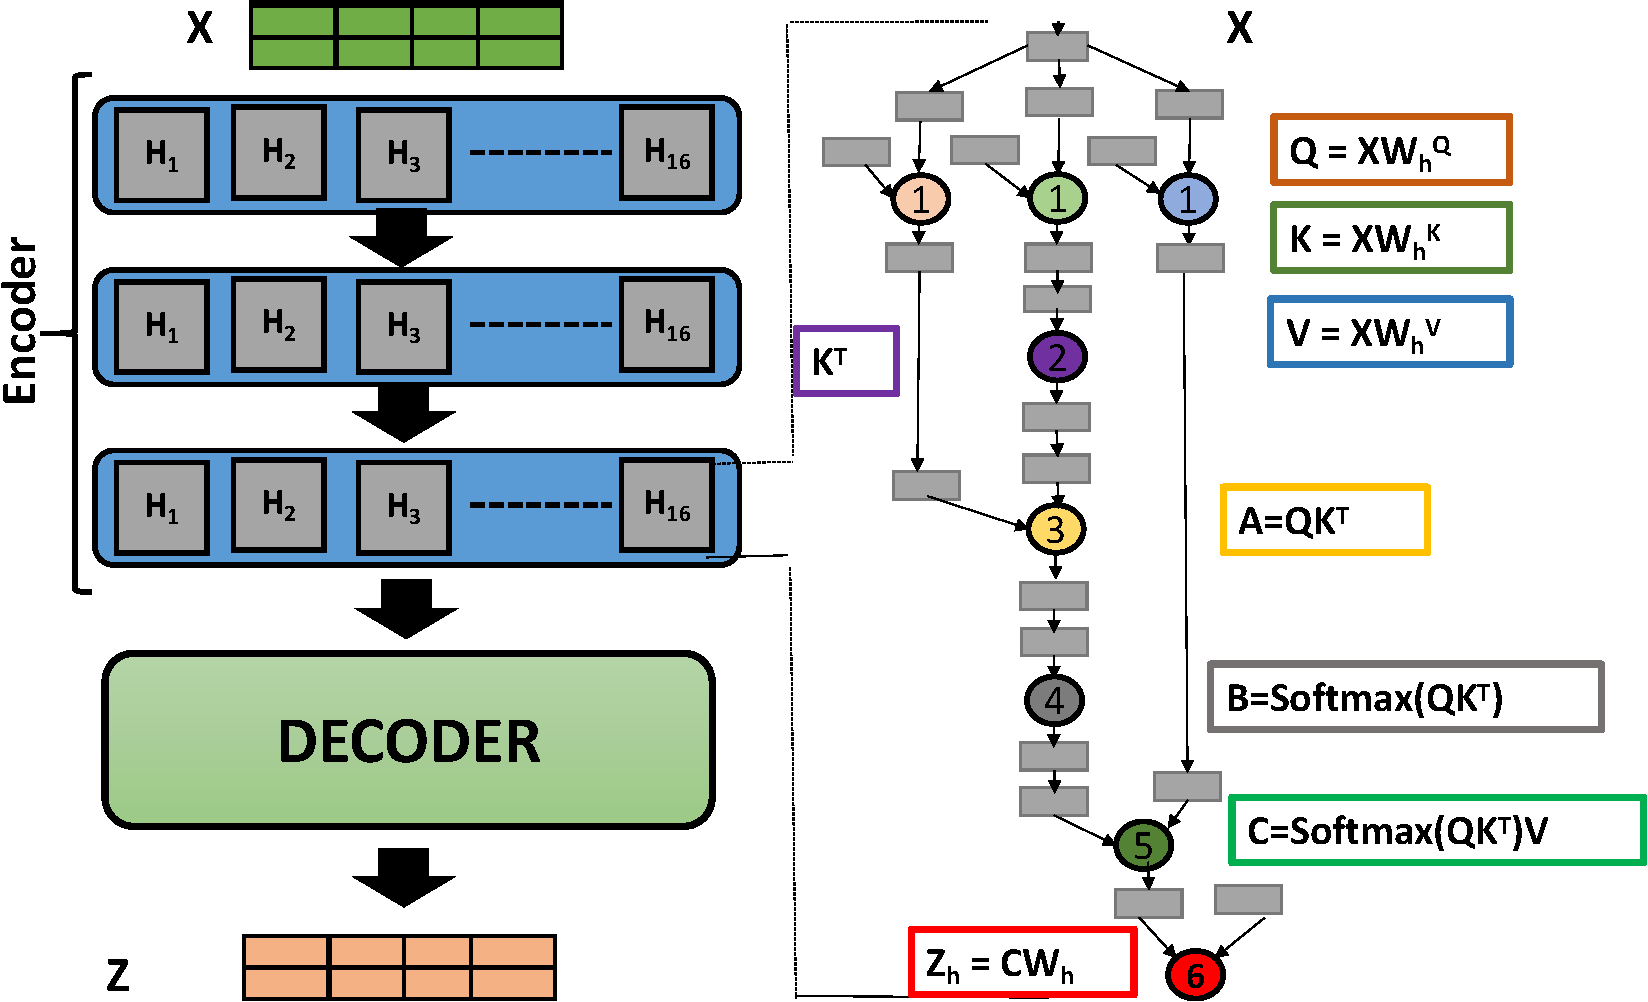
\includegraphics[scale=0.325]{Pictures/TransformerArch.pdf}
		\caption{\small Transformer Architecture\label{fig:transformer}}
	\end{figure}
	\par We conduct a series of experiments classified into three broad categories and for each experiment we define $\beta$ as the size of the transformer such that the matrices defined earlier $Q$,$K$,$V$,$X$ are all of dimensions $\beta \times \beta$. We denote the number of heads for the transformer as $H$. 
	\section{Experiment 1: Exhaustive Profiling}
	For Experiment 1, we profile one layer of the transformer architecture where we fix $\beta$ as 256 and vary the number of heads $H \in [1,16]$. Our experiment set is therefore a total of 16 input DAGs with each DAG representing a layer of a transformer neural network having $H\in[1,16]$ heads. 
	\par For each input DAG, we specify the task component mappings beforehand using the {\tt dev} guidance parameter for each kernel in the specification file. Given the structure of the DAG, it makes sense to cluster all kernels belonging to one transformer head into a task component and map it to a particular device. Since, the transformer heads are independent, such task component mappings would result in  there being no intra-edge buffers. As a result there will be no read callbacks. Thus for any transformer with $H$ heads, possible mapping configurations would be to 1) map all heads to a GPU device, 2) map 1 head to the CPU and $H-1$ heads to the GPU device, ... and finally $H+1$) mapping all $H$ heads to the GPU device.  Since each head is identical, clustering each head into a task component would result in a total of $H+1$ mapping configurations for a DAG with $H$ heads.
	\par We implement a static fine-grained scheduling heuristic called {\em clustering} specifically for any given transformer DAG with $H$ number of heads. Each task component $T_d$ represents one head and is annotated with the maximum bottom level rank defined in Equation \ref{eqn:brank_kernel} of the kernels in $FRONT(T_d)$. The $select$ routine for {\em clustering }selects from a set of task components, the component that has the maximum rank. The bottom level rank for any kernel in a DAG represents the maximum time left to finish all kernels in the path starting from $k$ to the last task in the DAG. The procedure $schedule$ sets up $C_d$ command queues for each task component $T_d$ mapped to device $d$. The {\em clustering} scheme for the transformer DAG is therefore characterized by the architecture mapping configuration tuple $mc=\langle CQ_{gpu},CQ_{cpu},h_{cpu}\rangle$. The parameter $Q_{gpu}\in [0,5] $ denotes the number of command queues used for the GPU device for executing a task component. Similarly, $Q_{cpu} \in [0,5]$ represents the number of command queues used for the CPU device. By varying the number of command queues for the CPU and the GPU, we have a total of $5*5=25$  architectural configurations. The parameter $h_{cpu}$ represents  the number of task components to be mapped to the CPU device.  The remaining $H-h_{cpu}$ task components are mapped to the GPU device. We consider the default configuration to be the case when the entire DAG is mapped to the GPU device using a single command queue i.e. $mc=(1,0,0)$, which essentially represents a coarse-grained scheduling decision, since we are using only 1 command queue.
	\par  For each DAG distinguished by the number of heads $H$, the best mapping configuration for {\em clustering} is the one which gives the best  speedup with respect to time taken by the DAG to execute in its default configuration which is using 1 GPU device with 1 command queue i.e. $mc=(1,0,0)$. We profile a total of $(H+1)*5*5$ such mapping configurations for each transformer DAG with $H$ heads and highlight our observations in  Fig. \ref{fig:Expt1}. 
	\begin{figure}[ht]
		\centering
		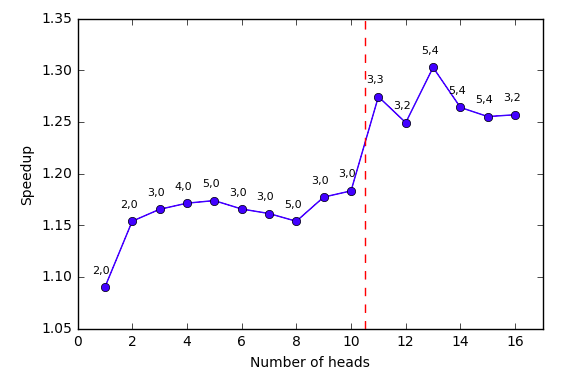
\includegraphics[scale=0.45]{Pictures/Expt-1.png}
		\caption{\small Speedup of best over default configuration \label{fig:Expt1}}
	\end{figure}
	The x-axis denotes the total number of heads for the transformer. The y-axis represents the speedups obtained for the best configuration for each DAG over the default configuration. Each point is labeled by the $CQ_{gpu},CQ_{cpu}$ tuple corresponding to the best configuration. We further note that for DAGs with number of heads upto 10 (region to the left of the dotted line), $h_{cpu}$ is 0. For DAGs having  number of heads greater than 10 (region to the right of the dotted line), we have $h_{cpu}=1$. 
	\par Thus, for DAGs with $H \in [1,10]$, we observe that the best configuration only differs from the default configuration with respect to the $CQ_{gpu}$ parameter. All the task components of the DAGs are scheduled to the GPU with the only difference being the number of command queues assigned to each component. The key observation in this region is that the transformer shows a clear speedup of about $15\% - 17\%$, if fine-grained scheduling is enabled leveraging multiple command queues. This highlights the effectiveness of automated fine-grained scheduling which our framework offers.
	\par For $H \in [11,16]$, we observe that scheduling one of the task components of the DAG to the CPU device yields the maximum speedups.  We also observe a jump in the relative speedup values as compared to the DAGs with $H <=10$. This is because apart from taking fine-grained scheduling decisions for the GPU device, we are also undertaking certain fine-grained scheduling decisions for the CPU device as well. This results in better extraction of application level-parallelism since mapping a task component to the CPU results in lesser contention for the GPU device. However, we observed that migrating more than one head does not yield better results. This may be attributed to the fact that overall execution of the transformer is bottlenecked by the time taken to execute kernels of a head on the CPU device. 
	\par We observe two key points from this experiment. Firstly, the transformer DAG is mapped efficiently using fine-grained scheduling decisions with the help of setting up multiple command queues, thereby lending credence to our framework's central idea of exploiting concurrency. Secondly, we observe that only for DAGs with $H > 10$, it is meaningful to utilise the CPU device for further speedups. This makes sense since i) the GPU has an order of magnitude number of processing elements greater than the CPU under consideration, ii) the kernels selected are optimized for GPUs rather than CPUs and iii) the CPU device is heavily engaged in setting up command queues and issuing directives to the devices in the heterogeneous platform.  Mapping more than 1 head for execution on the CPU actually takes more time to execute than that of mapping the remaining heads to the GPU device. 
	\par In the current experiment we consider specific DAG head mappings along with a choice of command queues and devices  based on what worked best for the given DAG and the given mapping configuration. Our next two categories of experiments consider typical dynamic heterogeneous scheduling policies like Eager-Scheduling and HEFT. We present a comparative evaluation between these methods and our clustering based static scheme in the context of the transformer DAG. 
		
	\section{Experiment 2: Clustering vs Eager Execution} We have implemented a simplistic eager execution based scheduling algorithm in our framework which is a dynamic scheduling scheme inspired from StarPU. For achieving this, we have implemented the $select$ routine to choose task components based on the bottom level ranks discussed earlier. Here, each task component represents one kernel in the DAG getting mapped to a device $d$ with one command queue.  For selecting devices, the $select$ routine selects any device that is available at runtime. Since, eager is a dynamic scheme, the choice of the device for execution is not known beforehand. This prohibits taking advantage of fine-grained scheduling decisions of interleaving data-transfers with execute operations.
	\begin{figure}[ht]
		\centering
		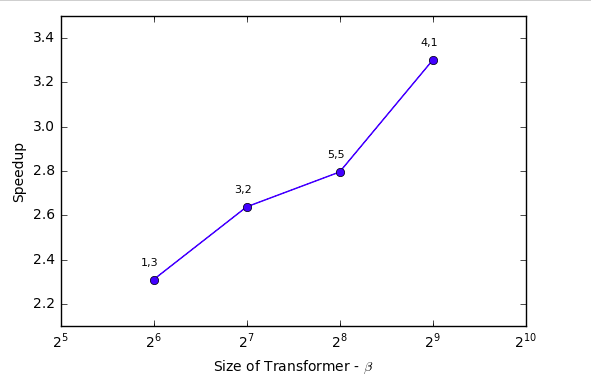
\includegraphics[scale=0.45]{Pictures/Expt-2.png}
		\caption{\small Clustering vs Eager \label{fig:Expt2}}
	\end{figure}
	\par For a comparative evaluation of this dynamic scheme with {\em clustering}, we generate a set of input DAGs by keeping the number of heads $H$ fixed to $16$ and by varying the size parameter $\beta$ from $64$ to $512$ in powers of 2. We profile each such input DAG, using both {\em eager} scheduling and {\em clustering} schemes for all possible mapping configurations. We compute the speedups of execution times taken by {\em clustering} based scheduling for the best mapping configuration  over that of {\em eager} and highlight them in Figure \ref{fig:Expt2}. 
	The x-axis represents the size of the transformer head ($\beta$) and the y-axis represents the speedup values. Each point in the plot is again labelled by the tuple $Q_{gpu},Q_{cpu}$ used by the best mapping configuration for the clustering scheme. The third element of the best configuration $H_{cpu}$ was found to be 1 for each $\beta$. It can be observed that {\em clustering} outperforms {\em eager} by a considerable margin. Since only one command queue per device is used, the scheduling scheme is restricted to taking coarse-grained scheduling decisions only and fails to take advantages of concurrency offered by fine-grained scheduling decisions. 
	\par We next perform a deeper analysis of the scheduling decisions taken by the two scheduling schemes for a DAG with $\beta=512$ using the Gantt charts for {\em eager} and {\em cluster} scheduling depicted in
	Figures \ref{fig:heft_gannt} and \ref{fig:best_gannt} respectively. The primary reason for the poor performance of  {\em eager} maybe attributed to the
	greedy nature of its dispatching mechanism. One can observe that multiple GEMM kernels have been scheduled on the CPU, thereby taking a significantly larger amount of time. The delay in  execution of the GEMM kernels in the first level stalls the entire progress of the DAG. 
	\section{Experiment 3: Clustering vs HEFT}
	We implement the standard Heterogeneous Earliest Finishing Time First algorithm using our framework whose primary principle is based on selecting kernels based on their bottom level ranks and dispatching to devices according to their estimated earliest finish times. Similar to {\em eager}, the scheduling heuristic {\em heft} assumes each task component to represent one kernel and sets up one command queue for each device. We override the $select$ routine such that each dispatch decision involves i) choosing the kernel $k$ with the maximum bottom level rank and for ii) choosing the device $d$ with the earliest finishing time (EFT). In our implementation, we calculate EFT of a device $d$ as the sum of the execution time of the kernel currently executing on $d$ and the execution time of the kernel to be dispatched on the device. Note, our implementation for HEFT is not calibrated to take into account scheduling overheads such as enqueuing delays while selecting devices. We again consider the same set of input DAGs used in Experiment 2 and plot the speedups of the best configurations of the clustering scheme over the {\em heft} scheme in  Figure \ref{fig:Expt3}.
	\begin{figure}[ht]
		\centering
		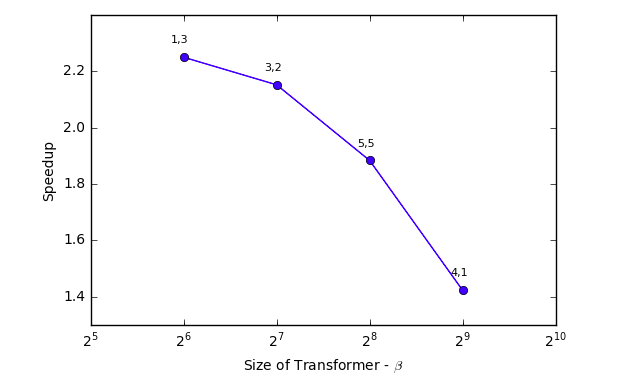
\includegraphics[scale=0.45]{Pictures/Expt-3.png}
		\caption{\small Clustering vs {\em heft} scheduling \label{fig:Expt3}}
	\end{figure}
	\par As expected, {\em heft} performs better than {\em eager} due to the prediction of earliest finishing times for each task.  However, {\em heft} being implemented as a dynamic scheme is short sighted and fails to exploit concurrency aware scheduling decisions undertaken by {\em clustering}. 
	\par We again perform a deeper analysis here between the scheduling decisions by plotting the Gantt chart for the DAG with $\beta = 512$ in Fig. \ref{fig:heft_gannt}. In contrast to {\em eager} scheduling, {\em heft} exclusively uses the GPU for the GEMM kernels and it thus approximately $2.4 \times$ faster than eager. 
	\par We next list a set of general observations explaining as to why our static clustering scheme performed better than that of the dynamic schemes {\em eager} and {\em heft}. From the gantt charts we may observe that kernels scheduled using our {\em clustering} scheme start much later when compared to kernels being scheduled in the other schemes. This may be attributed to the fact, that our framework sets up the command queues first with operations pertaining to all kernels in a task component  before actually scheduling the kernels to their respective devices. As a result, we can see that there exist no gaps between the execution of two kernels in our scheduling scheme.
	For the other two policies, despite being dynamic in nature, they have to rely on read callbacks to make dispatch decisions. Naturally, since read callbacks perform exclusive thread-safe updates, the successor kernels need to wait before getting dispatched. Furthermore, we can observe the gaps for the kernels scheduled to the GPU device to be more. This makes sense, since the callback function is initiated as a daemon thread by the OpenCL runtime system. The scheduler thread may be swapped out of main memory at that point of time by the operating system. The scheduler thread must resolve these updates first before dispatching the successor kernels. The successive gaps introduced between each kernel execution in the DAG results in a considerable slowdown when compared to the scheduling decisions employed by {\em clustering}. 
	\begin{figure}[ht]
		\centering
		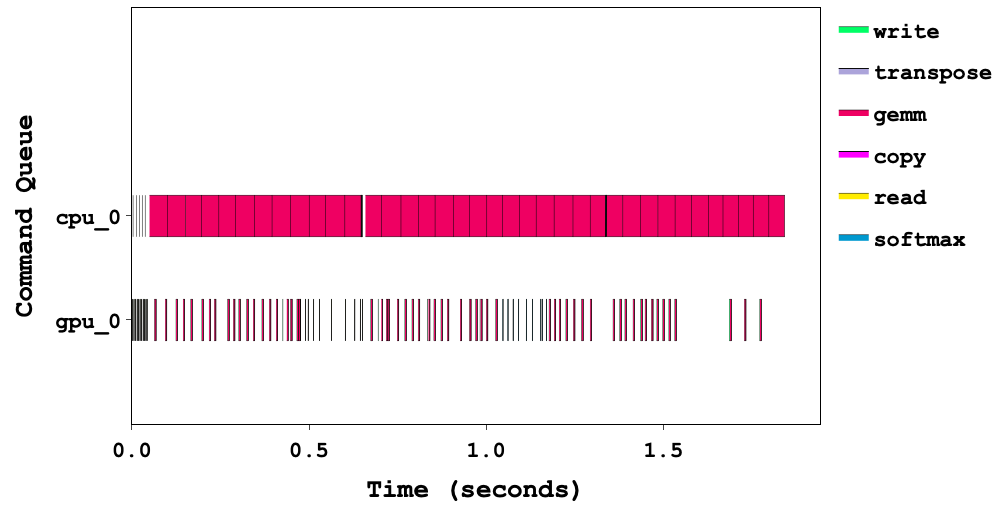
\includegraphics[scale=0.40]{Pictures/eager_gannt.png}
		\caption{\small Gannt chart for {\em eager} scheduling \label{fig:eager_gannt}}
	\end{figure}
	\begin{figure}[ht]
		\centering
		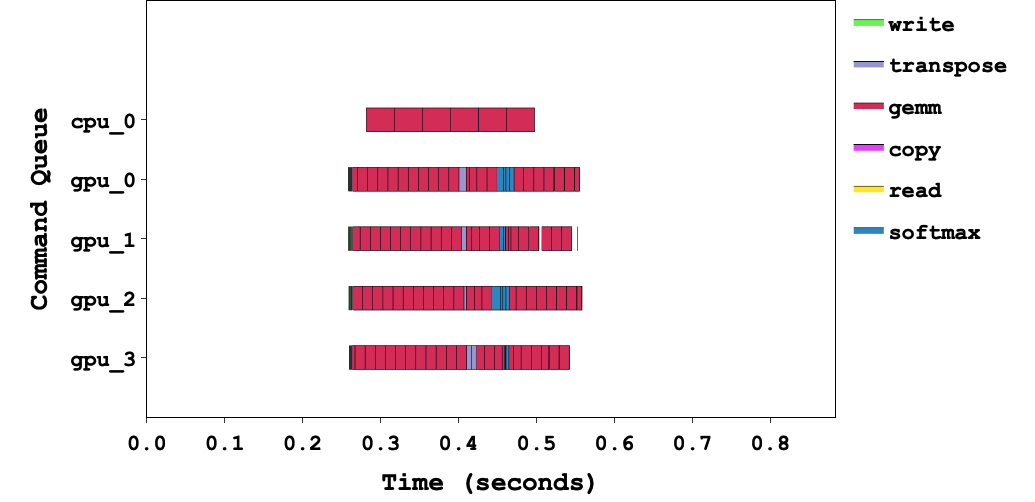
\includegraphics[scale=0.40]{Pictures/best_gannt.png}
		\caption{\small Gannt chart for {\em cluster} scheduling  \label{fig:best_gannt}}
	\end{figure}
	\begin{figure}
		\centering
		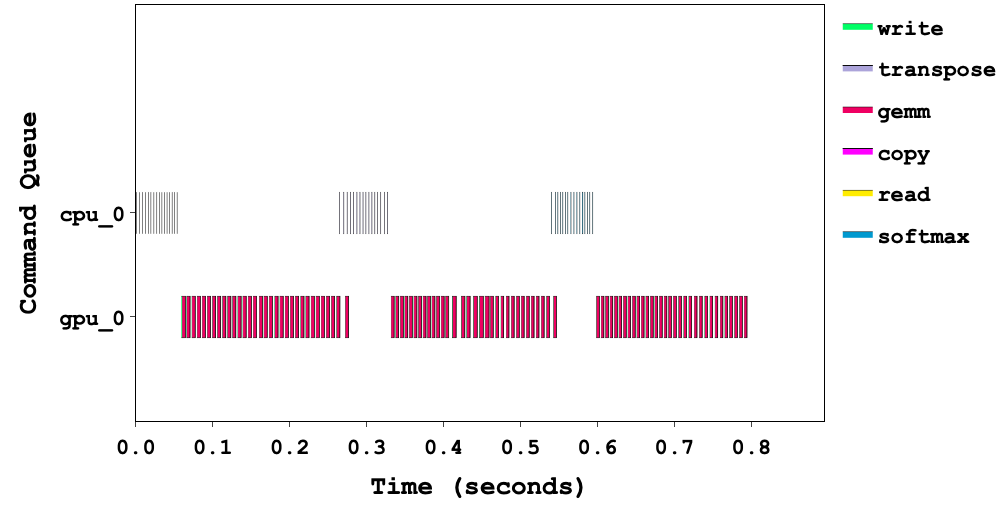
\includegraphics[scale=0.40]{Pictures/dynamic_heft_gannt.png}
		\caption{\small Gannt chart for {\em heft} scheduling \label{fig:heft_gannt}}
	\end{figure}
	Thus, we empirically establish the necessity for static cluster based scheduling policies for the transformer neural networks using these experiments. In general, for any application exhibiting potential scope for concurrency, scheduling schemes must be envisaged that take into account i)fine-grained scheduling decisions with respect to the structure of the DAG as well as ii) intricate runtime environment delays occurring as a result of enqueuing commands and processing simultaneous callback events. 